% !TEX root = ../om_ts_02.tex

\begin{frame} % название фрагмента

\videotitle{ETS(AAN)}

\end{frame}



\begin{frame}{ETS(AAN): план}
  \begin{itemize}[<+->]
    \item Наконец-то настоящий тренд!
    \item Формулы для прогнозов.
    \item Немного подробностей о правдоподобии.
  \end{itemize}

\end{frame}


\begin{frame}
  \frametitle{Настоящий тренд!}

  $y_t$ — наблюдаемый ряд;

  $\ell_t$ — тренд, очищенный ряд (\alert{единорог});

  $b_t$ — текущая скорость роста очищенного ряда (\alert{единорог});

  $u_t$ — случайная ошибка.

  \pause
  ETS(AAN):

  A — \alert{аддитивная} ошибка;

  A — \alert{аддитивный} тренд;

  N — \alert{нет} сезонности. 

\end{frame}


\begin{frame}
  \frametitle{ETS(AAN): уравнения}

  
  \[
    \begin{cases}
     y_t = \ell_{t-1} + \alert{b_{t-1}} + u_t; \\
    \ell_t = \ell_{t-1} + \alert{b_{t-1}} + \alpha u_t, \text{ стартовое } \ell_0; \\
    u_t \sim \dN(0;\sigma^2) \text{ и независимы.} \\
    \alert{b_t = b_{t-1} + \beta u_t},\text{ стартовое } b_0; \\
    \end{cases}
  \]

  \pause
  Параметры: $\alpha$, $\beta$, $\sigma^2$, $\ell_0$, $b_0$.
  

\end{frame}

\begin{frame}
  \frametitle{ETS(AAN): прогнозируем}

  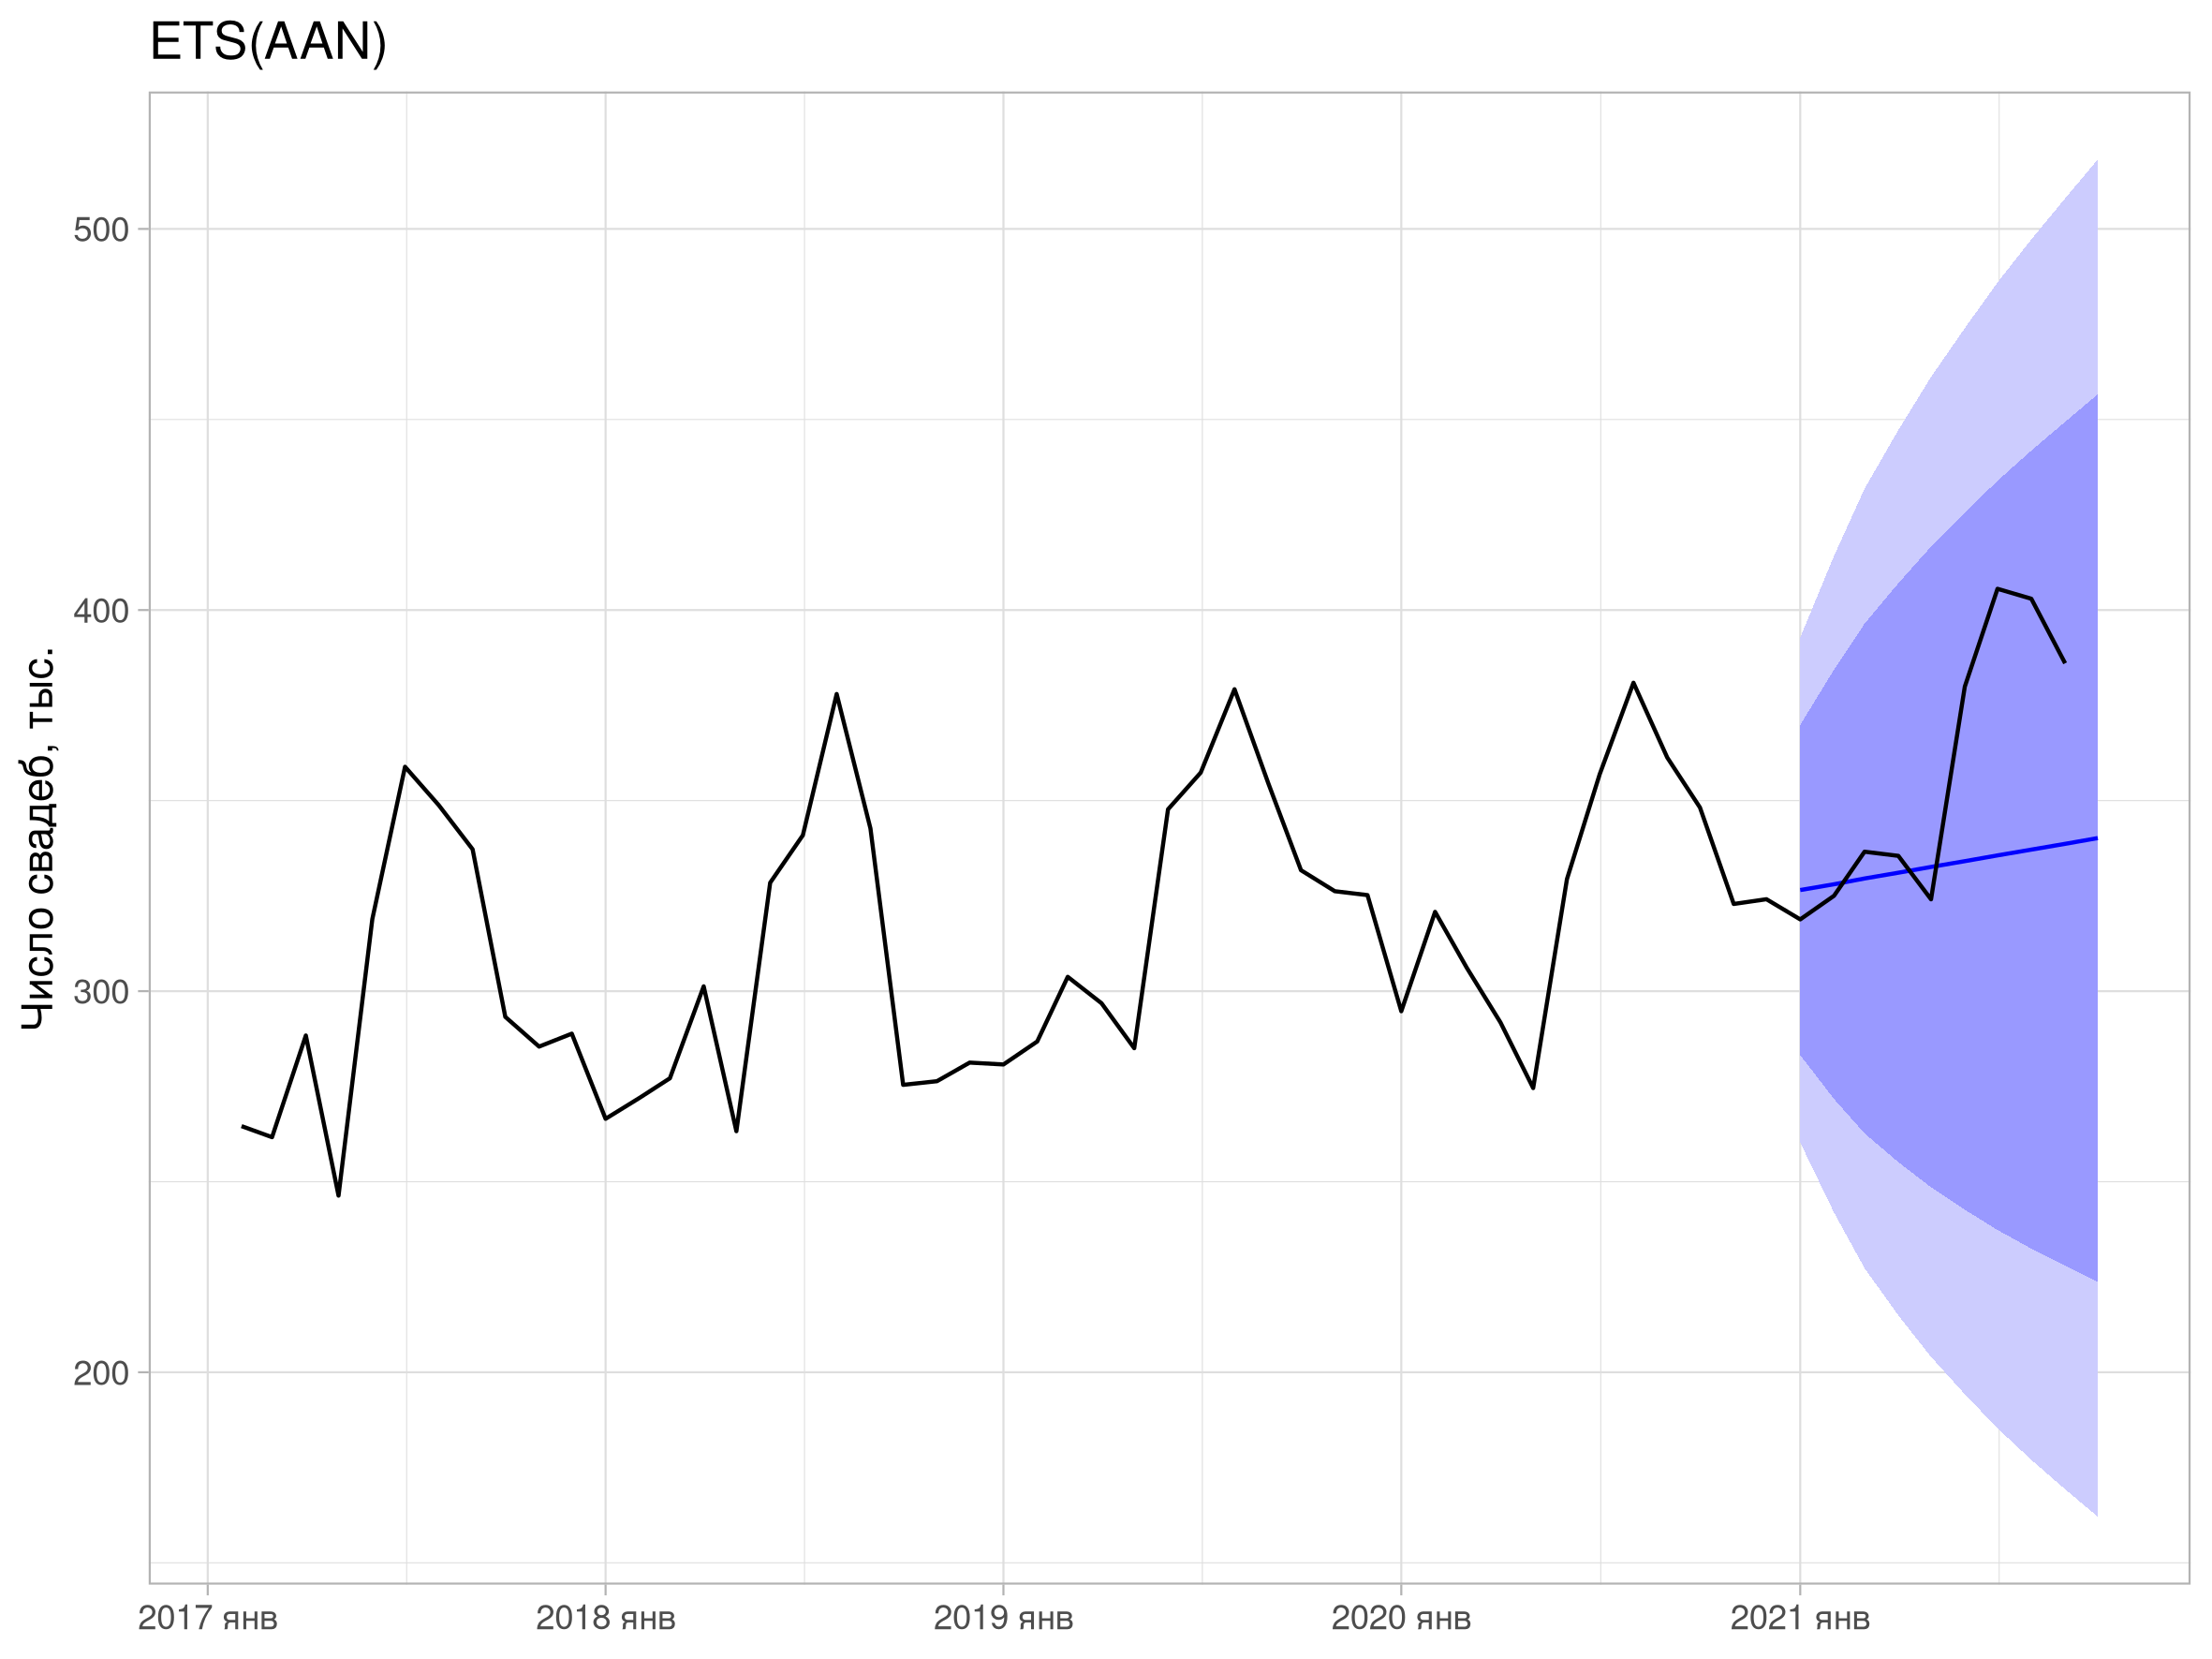
\includegraphics[width=\textwidth]{pictures/om_ts_02-052.png}

\end{frame}


\begin{frame}
  \frametitle{Прогноз на 1 шаг вперёд}

  \[
      \begin{cases}
        y_t = \ell_{t-1} + b_{t-1} + u_t; \\
       \ell_t = \ell_{t-1} + b_{t-1} + \alpha u_t, \text{ стартовое } \ell_0; \\
       u_t \sim \dN(0;\sigma^2) \text{ и независимы.} \\
       b_t = b_{t-1} + \beta u_t,\text{ стартовое } b_0; \\
       \end{cases}
  \]
  \pause
\[
y_{T+1} = \ell_T + b_T + u_{T+1}  
\]
\pause
\[
  (y_{T+1} \mid \mathcal F_T) \sim \dN(\ell_T + b_T; \sigma^2)  
\]

\end{frame}


\begin{frame}
  \frametitle{Прогноз на 2 шага вперёд}

  \[
    \begin{cases}
      y_t = \ell_{t-1} + b_{t-1} + u_t; \\
     \ell_t = \ell_{t-1} + b_{t-1} + \alpha u_t, \text{ стартовое } \ell_0; \\
     u_t \sim \dN(0;\sigma^2) \text{ и независимы.} \\
     b_t = b_{t-1} + \beta u_t,\text{ стартовое } b_0; \\
     \end{cases}
   \]
  \pause
  \begin{multline*}
    y_{T+2} = \ell_{T+1} + b_{T+1} + u_{T+2} = (\ell_T + b_T + \alpha u_{T+1}) +\\
    + (b_T + \beta u_{T+1}) + u_{T+2} 
  \end{multline*}
   \pause
  \[
  (y_{T+2} \mid \mathcal F_T) \sim \dN(\ell_T + 2b_T; \sigma^2((\alpha + \beta)^2 + 1))
  \]
  
\end{frame}


\begin{frame}
  \frametitle{Детали правдоподобия}
  \alert{Функция правдоподобия}:
  \begin{multline*}
    \ln L(y \mid \theta) = \ln L(y_1 \mid \theta) + \ln L(y_2 \mid y_1, \theta) + \ldots + \\
     + \ln L(y_T \mid y_{T-1}, \ldots, y_1, \theta),
  \end{multline*}

  где $\theta = (\alpha, \beta, \sigma^2, \ell_0, b_0)$.

  \pause
  Уравнения для эволюции $y_t$, $b_t$, $\ell_t$ — \alert{линейные}.
  
  \pause
  \[
  (y_t \mid \mathcal F_{t-1}) \sim \dN(\ell_{t-1} + b_{t-1}; \sigma^2)
  \]

  \pause
  \[
  \ln L(y_t \mid \mathcal F_{t-1}) = 
  \ln \frac{1}{\sqrt{2\pi \sigma^2}} - \frac{1}{2\sigma^2} (y_t - (\ell_{t-1} + b_{t-1}))^2
  \]

\end{frame}


\begin{frame}{ETS(AAN): итоги}

  \begin{itemize}[<+->]
    \item Настоящий \alert{тренд в модели}. 
    \item Наклон линии тренда может меняться.
    \item Устройство функции правдоподобия.
  \end{itemize}
\end{frame}



